\documentclass[a4paper]{article}

%\setlength{\parskip}{0.5\baselineskip}

\usepackage{geometry}
\geometry{left = 2.54 cm, right = 2.54 cm, top = 2.54 cm, bottom = 2.54 cm}

\usepackage{setspace}
\renewcommand{\baselinestretch}{1.0}
\usepackage{indentfirst}
\setlength{\parindent}{2em}

%\usepackage{fontspec}
%\setmainfont{Times New Roman}

\usepackage[]{cprotect}

\usepackage{hyperref}
\hypersetup{
  colorlinks=true,
  linkcolor=blue,
  filecolor=magenta,
  urlcolor=cyan,
}

\usepackage{ulem}
\usepackage{graphicx}
%\usepackage{wrapfig}
\usepackage{enumitem}
%\usepackage{xcolor}
\usepackage{subcaption}
\usepackage{float}
\usepackage{amsmath, amssymb, amsthm}
\usepackage{booktabs}

%\pagestyle{empty} % Not showing page number

\begin{document}
\renewcommand{\thesection}{\Roman{section}}
\renewcommand{\thesubsection}{\Alph{subsection}}
\renewcommand{\thesubsubsection}{\thesubsection.\arabic{subsubsection}}
\renewcommand{\d}{\: \mathrm{d} }
\newcommand{\e}{\mathrm{e}}

\begin{center}
  \textbf{\Large VE373 Recitation Class}\\[1em]
  \textbf{\large Week 2} \\[1em]
  2022.05.21 \\[1em]
\end{center}

\section*{L1 --- Introduction to Embedded Systems}
  \begin{enumerate}[label = \arabic*.]
    \item \textbf{Microprocessor (MPU) \& Microcontroller (MCU)}
      \begin{figure}[H]
        \centering
        \begin{subfigure}[b]{0.65\linewidth}
          \centering
          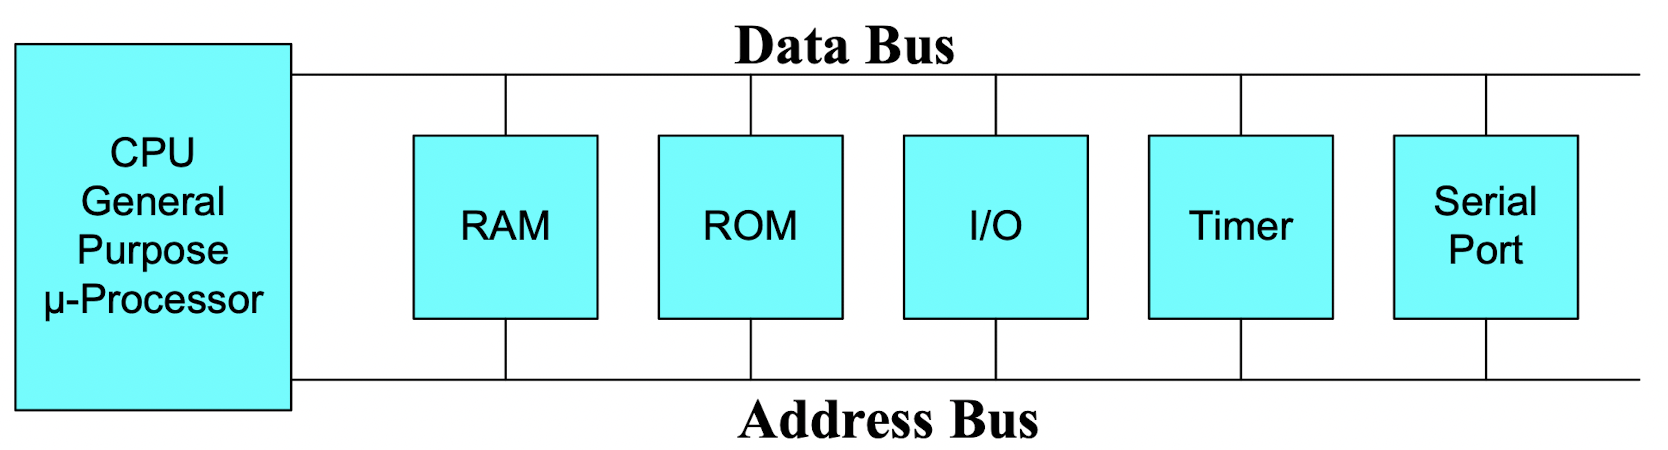
\includegraphics[width=0.9\linewidth]{MPU.png}
          \caption{Microprocessor}
          \label{subfig:MPU.png}
        \end{subfigure}
        \begin{subfigure}[b]{0.3\linewidth}
          \centering
          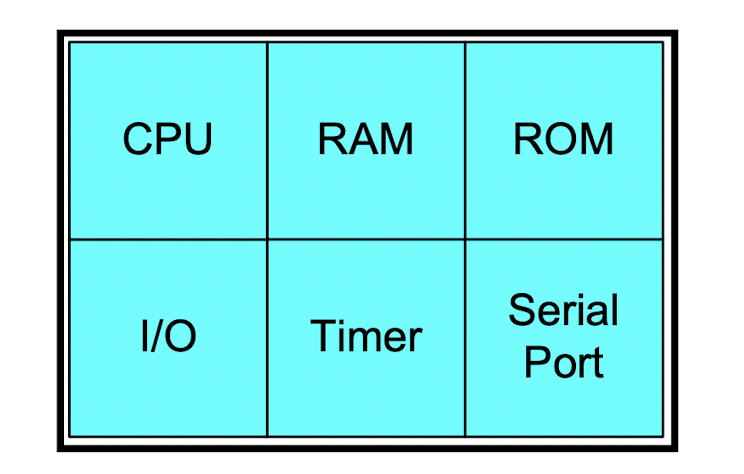
\includegraphics[width=0.9\linewidth]{MCU.png}
          \caption{Microcontroller}
          \label{subfig:MCU.png}
        \end{subfigure}
      \end{figure}

      \begin{table}[H]
        \centering
        \begin{tabular}{p{0.45\linewidth} p{0.45\linewidth}}
          \toprule
          \multicolumn{1}{c}{\textbf{Microprocessor}}                                                                                                             & \multicolumn{1}{c}{\textbf{Micro Controller}}                                                                                                    \\
          \midrule
          Microprocessor is heart of Computer system.                                                                                                             & Micro controller is a hear of embedded system.                                                                                                   \\
          \midrule
          \textbf{It is just a processor. Memory and I/O components have to be connected externally.}                                                             & \textbf{Micro controller has external processor along with internal memory and I/O components.}                                                  \\
          \midrule
          The circuit is large.                                                                                                                                   & The circuit is small.                                                                                                                            \\
          \midrule
          Cannot be used in compact systems and hence inefficient.                                                                                                & Can be used in compact systems and hence it is an efficient technique.                                                                           \\
          \midrule
          Cost of the entire system increases.                                                                                                                    & Cost of the entire system is low.                                                                                                                \\
          \midrule
          Due to external components, the entire power consumption is high. Hence it is not suitable to used with devices running on stored power like batteries. & Since external components are low, total power consumption is less and can be used with devices running on stored power like batteries.          \\
          \midrule
          Most of the microprocessors do not have power saving features.                                                                                          & Most of the micro controllers have power saving modes like idle mode and power saving mode. This helps to reduce power consumption even further. \\
          \midrule
          Since memory and I/O components are all external, each instruction will need external operation, hence it is relatively slower.                         & Since components are internal, most of the operations are internal instruction, hence speed is fast.                                             \\
          \midrule
          Microprocessor have less number of registers, hence more operations are memory based.                                                                   & Micro controller have more number of registers, hence the programs are easier to write                                                           \\
          \midrule
          Microprocessors are based on Von Neumann model/architecture where program and data are stored in same memory module.                                    & Micro controllers are based on Harvard architecture where program memory and Data memory are separate.                                           \\
          \midrule
          Mainly used in personal computers.                                                                                                                      & Used mainly in washing machines, MP2 players.                                                                                                    \\
          \bottomrule
        \end{tabular}
        \label{tab:MCU_MPU}
      \end{table}

    \item \textbf{Von Neumann \& Havard Architecture}
      \begin{figure}[H]
        \centering
        \begin{subfigure}[b]{0.45\linewidth}
          \centering
          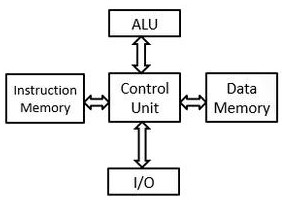
\includegraphics[width=0.9\linewidth]{Harvard_architecture.jpeg}
          \caption{Harvard Architecture}
          \label{subfig:Harvard_architecture.jpeg}
        \end{subfigure}
        \begin{subfigure}[b]{0.45\linewidth}
          \centering
          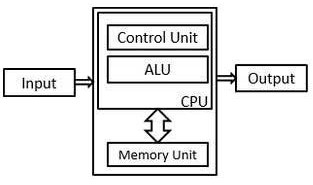
\includegraphics[width=0.9\linewidth]{Von_neumann_architecture.jpeg}
          \caption{Von Neumann Architecture}
          \label{subfig:Von_neumann_architecture.jpeg}
        \end{subfigure}
      \end{figure}

      \begin{table}[H]
        \centering
        \begin{tabular}{p{0.45\linewidth} p{0.45\linewidth}}
          \toprule
          \multicolumn{1}{c}{\textbf{Harvard architecture}}                       & \multicolumn{1}{c}{\textbf{Von Neumann architecture}}                       \\
          \midrule
          \textbf{It required two memories for their instruction and data.}       & \textbf{It required only one memory for their instruction and data.}        \\
          \midrule
          Harvard architecture is required separate bus for instruction and data. & Von Neumann architecture is required only one bus for instruction and data. \\
          \midrule
          Processor can complete an instruction in one cycle                      & Processor needs two clock cycles to complete an instruction.                \\
          \midrule
          Easier to pipeline, so high performance can be achieve.                 & Low performance as compared to Harvard architecture.                        \\
          \midrule
          Comparatively high cost.                                                & It is cheaper.                                                              \\
          \bottomrule
        \end{tabular}
        \label{tab:von_neumann_havard}
      \end{table}
  \end{enumerate}

\section*{L2 --- PIC MCU Architecture}
  \begin{enumerate}[label = \arabic*.]
    \item \textbf{PIC32}
      \begin{figure}[H]
        \centering
        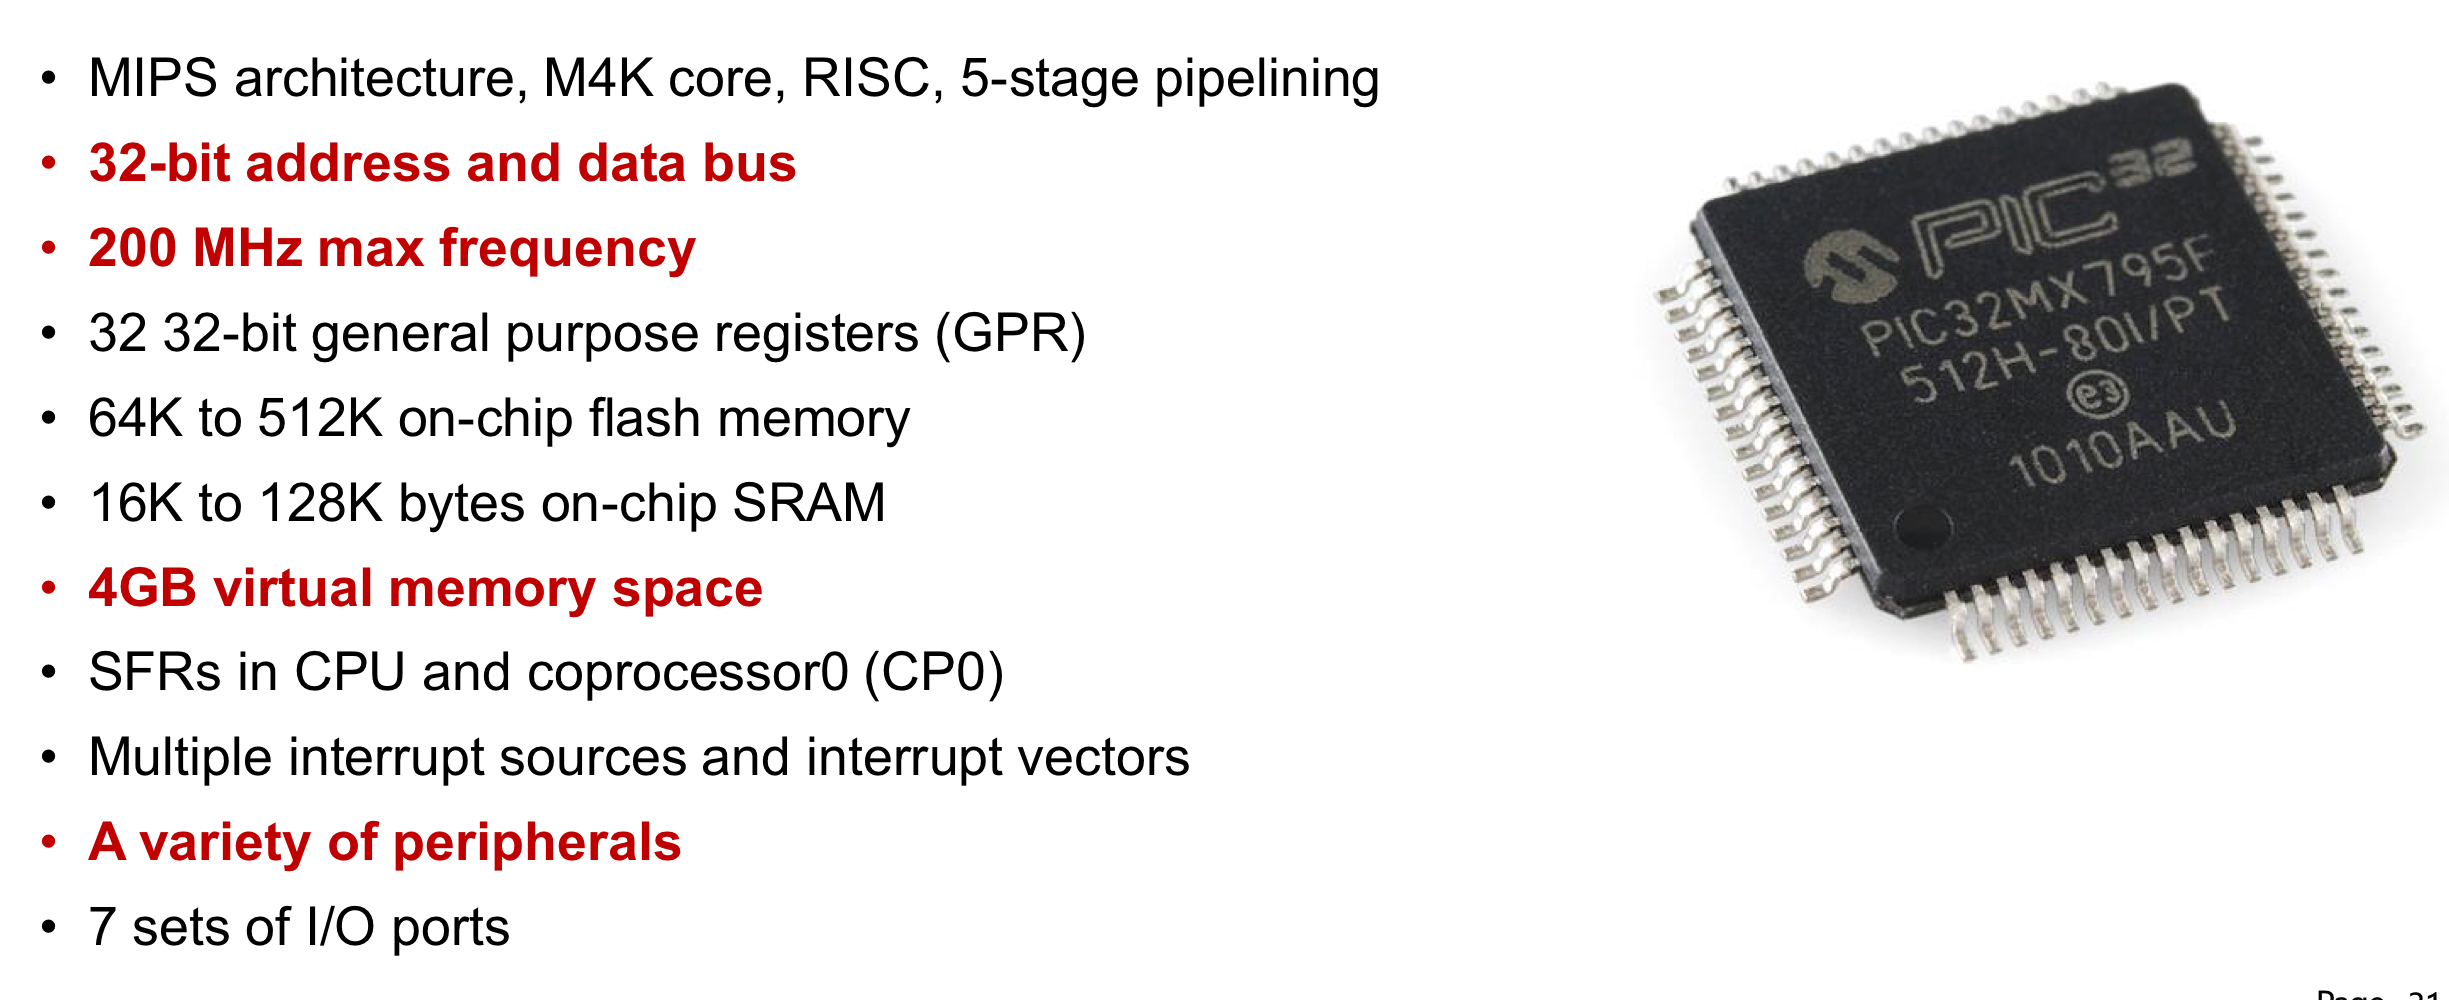
\includegraphics[width=0.9\linewidth]{PIC32_MCU_Architecture_specification.jpeg}
        \caption{32-bit PIC32 MCU Example: Architecture}
        \label{fig:PIC32_MCU_Architecture_specification.jpeg}
      \end{figure}

      \par \( n \)-bit data address bus = support up to \( 2^n \) byte memory.

      \par PIC32 is a combination of Von Neumann and Hasrvard architecture. See \href{https://blog.flyingpic24.com/2008/10/26/pic32-harvard-or-von-neumann/}{here} for more details if interested.
    \item \textbf{Special Function Register}
      \par Used to config, control and monitor various aspects of the microprocessor's function.
      \par For example, \verb|T1CON|, \verb|TMR1| and \verb|PR1| when using Timer 1.
  \end{enumerate}

\section*{L3 --- Embedded Programming}
  \begin{enumerate}[label = \arabic*.]
    \item \textbf{Compiler}
      \begin{figure}[H]
        \centering
        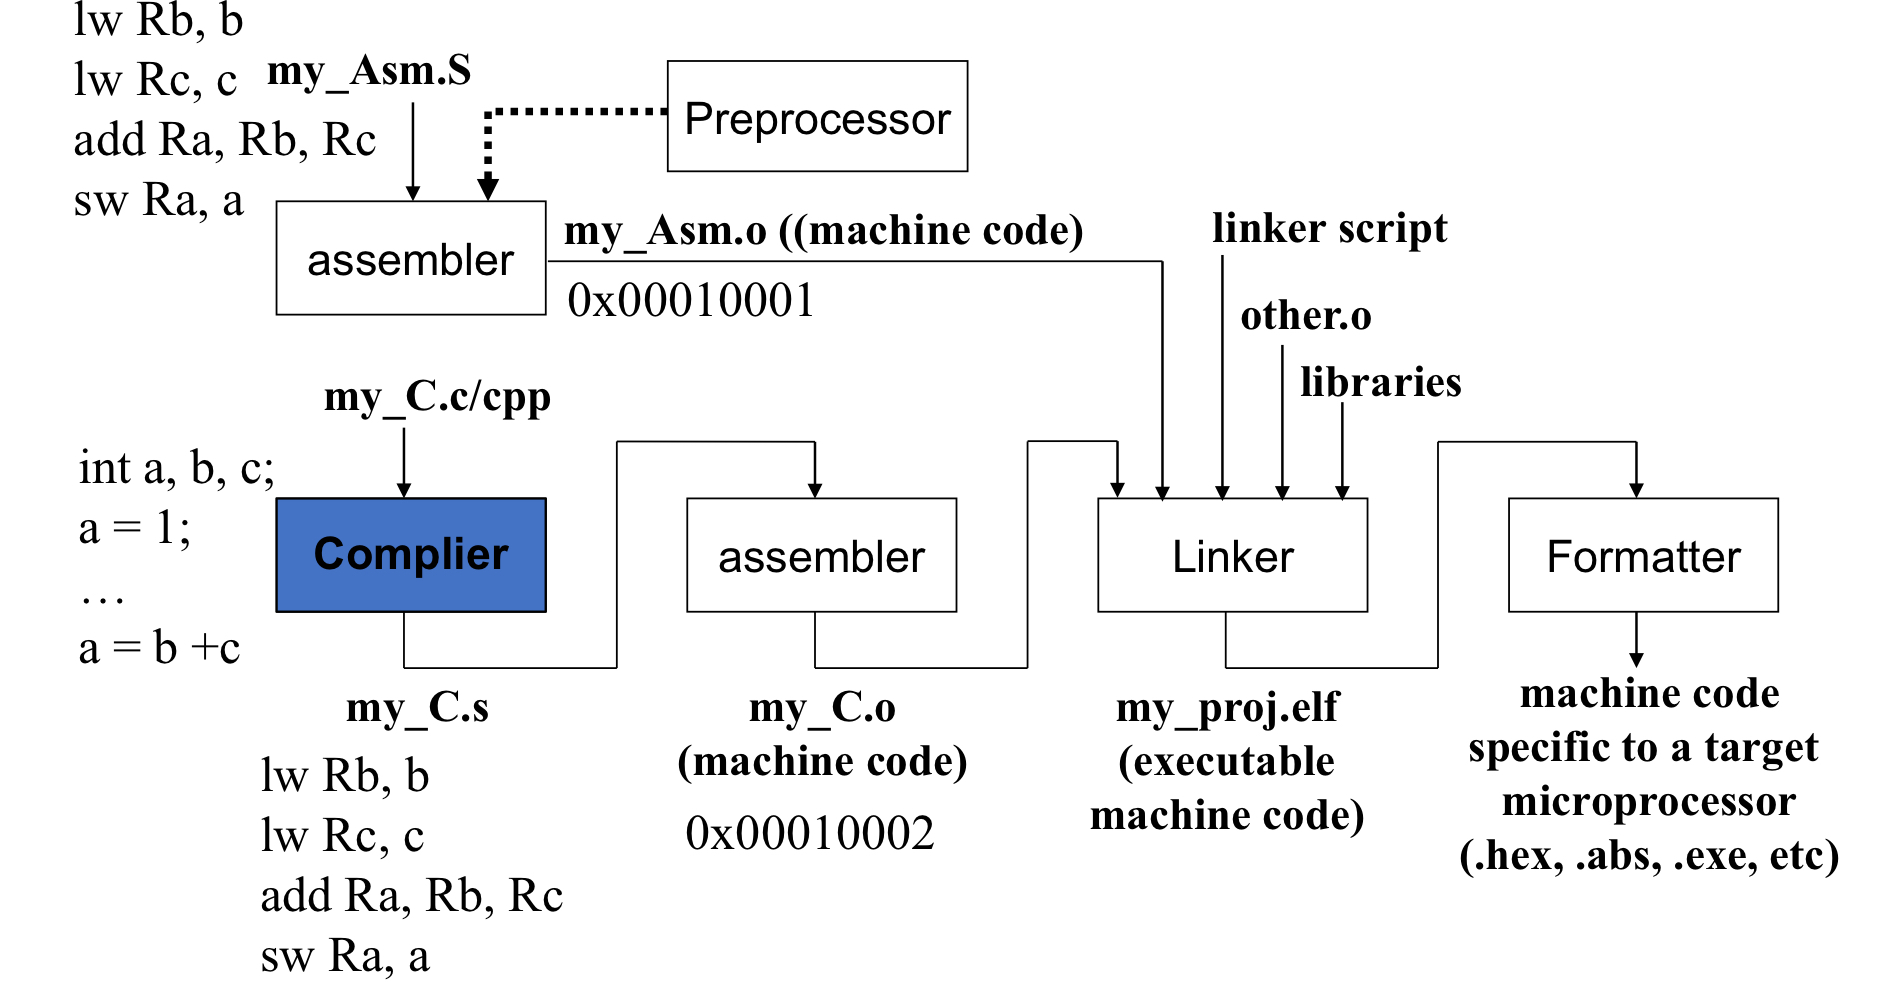
\includegraphics[width=0.9\linewidth]{Program_build_flow.jpeg}
        \caption{Workflow}
        \label{fig:Program_build_flow.jpeg}
      \end{figure}

    \item \textbf{Const \& Volatile}
      \begin{itemize}[leftmargin = 1cm]
        \item const: the value not supposed to be written by program (read only).
        \item volatile: the value can be changed by something other than program so it should be reexamined frequently.
      \end{itemize}
    \item \textbf{Directives}
      \par Directives: compiler dependent commands.
      \par e.g. \verb|#pragma interrupt func_name ipln| (will be used later).
  \end{enumerate}

\section*{L4 --- Timers and IO}
  \begin{enumerate}[label = \arabic*.]
    \item \textbf{Oscillator}
      \begin{itemize}[leftmargin = 1cm]
        \item \textbf{Internal oscillator}:
          \begin{itemize}[leftmargin = 1cm]
            \item Integrated on-chip within the processor
            \item Low frequency accuracy and stability.
            \item Most of internal oscillator are RC circuits
          \end{itemize}
        \item \textbf{External oscillator}
          \begin{itemize}[leftmargin = 1cm]
            \item Located off-chip on the PCB
            \item High frequency accuracy and stability
            \item Most of external oscillator are crystal oscillator
          \end{itemize}
      \end{itemize}

      \par Peripherals don't have a high clock frequency:
      \begin{itemize}[leftmargin = 1cm]
        \item No need
        \item Limited by parasitics
        \item Power consumption
      \end{itemize}
    \item \textbf{Timer}
      \par Two types, five timers on PIC32:
      \begin{itemize}[leftmargin = 1cm]
        \item Type A --- Timer 1
          \begin{itemize}[leftmargin = 1cm]
            \item \textcolor{red}{16-bit} synchronous/\textcolor{red}{asynchronous} timer/event counter
            \item Internal or external clock source
            \item Gated external event timer
          \end{itemize}
        \item Type B --- Timer 2, 3, 4, 5
          \begin{itemize}[leftmargin = 1cm]
            \item \textcolor{red}{16/32-bit} synchronous timer/event counter
            \item Internal or external clock source
            \item Gated external event timer
          \end{itemize}
      \end{itemize}
      \begin{figure}[H]
        \centering
        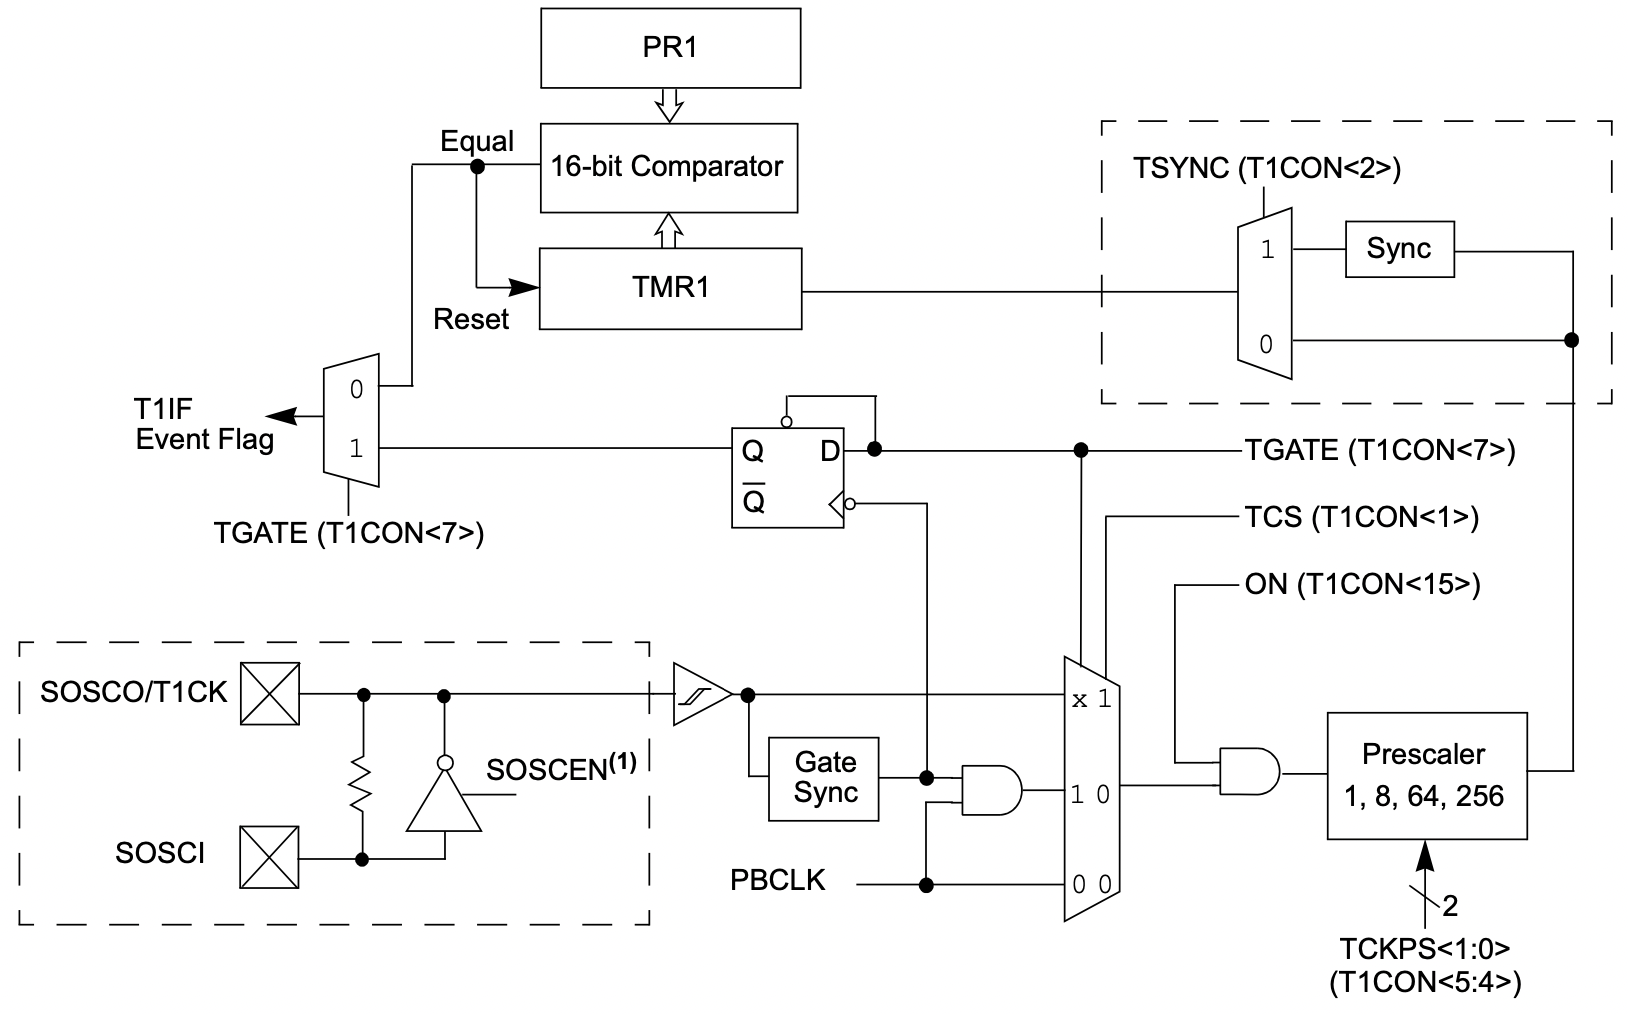
\includegraphics[width=0.9\linewidth]{Timer1_block_diagram.png}
        \caption{Timer 1 block diagram (Datasheet Page.~197)}
        \label{fig:Timer1_block_diagram.png}
      \end{figure}

    \item \textbf{16-bit synchronous timer setup steps}
      \par Use internal clock source --- \verb|PBCLK| as example.
      \begin{enumerate}[label = \arabic*.]
        \item Clear control bit \verb|ON| (\verb|TxCON<15>=0|) to disable timer.
        \item Clear control bit \verb|TCS| (\verb|TxCON<1>=0|) to select internal clock source \verb|PBCLK|.
        \item Select desired clock prescale value.
        \item Load/clear timer register \verb|TMRx| to specify initial counting value.
        \item Load period register \verb|PRx| with desired 16-bit match value.
        \item If interrupts used:
          \begin{enumerate}[label = \roman*.]
            \item Clear interrupt flag bit
            \item Configure interrupt priority and subpriority levels
            \item Set interrupt enable bit
          \end{enumerate}
        \item Set control bit \verb|ON| (\verb|TxCON<15>=1|) to start timer
      \end{enumerate}

  \end{enumerate}
\end{document}